\documentclass[12pt]{amsart}
\usepackage[T1]{fontenc}
\usepackage[utf8]{inputenc}

\usepackage[top=1.95cm, bottom=1.95cm, left=2.35cm, right=2.35cm]{geometry}

\usepackage{amsmath}
\usepackage{amssymb}
\usepackage{enumitem}
\usepackage{multicol}
\usepackage[french]{babel}
\usepackage[
    type={CC},
    modifier={by-nc-sa},
	version={4.0},
]{doclicense}

\usepackage{tnsmath}

\DeclareMathOperator{\taille}{\tau}

\newtheorem{fact}{Fait}
\newtheorem*{proof*}{Preuve}

\setlength\parindent{0pt}


\newcommand\squote[1]{\og #1 \fg{}}


\begin{document}

\title{BROUILLON - Tracé mécanique d'une hyperbole}
\author{Christophe BAL}
\date{DD MMMM YYYY}
\maketitle


\begin{center}
	\itshape
	Document, avec son source \LaTeX, disponible sur la page

	\url{https://github.com/bc-writings/bc-public-docs/tree/main/drafts}.
\end{center}


\bigskip


\begin{center}
	\hrule\vspace{.3em}
	{
		\fontsize{1.35em}{1em}\selectfont
		\textbf{Mentions \og légales \fg}
	}

	\vspace{0.45em}
	\doclicenseThis
	\hrule
\end{center}



\setcounter{tocdepth}{2}
\tableofcontents




\newpage

\section{\texorpdfstring{Comment additionner des nombres grâce à l'hyperbole d'équation $y = \frac{1}{x}$}%
                        {Comment additionner des nombres grâce à l'hyperbole d'équation y = 1/x}}

Dans un repère orthogonal, donnons nous la parabole $\setgeo{P} : y = x^2$ . Plaçons-y les points $A$ , $B$ et $S$ d'abscisses respectives $a$ , $b$ et  $s = a + b$ .
Observez
\footnote{
	Le lieu de téléchargement de ce document contient un fichier GeoGebra \texttt{base-tool.ggb} manipulable dynamiquement pour vérifier combien il est aisé de conjecturer quelque chose.
}
les trois cas ci-dessous et essayez de conjecturer quelque chose \emph{(la réponse est donnée dans la page suivante)}
\footnote{
	On peut géométriquement additionner modulo $2 \pi$ sur un cercle.
	Or $x^2 - y^2$ et $x^2 - y$ sont des formes quadratiques avec des propriétés géométriques communes.
	C'est là l'origine de la recherche proposée ici.
}.


\vspace{2.5em}

\begin{multicols}{2}
	\center
	\footnotesize
	\itshape
	
	\fbox{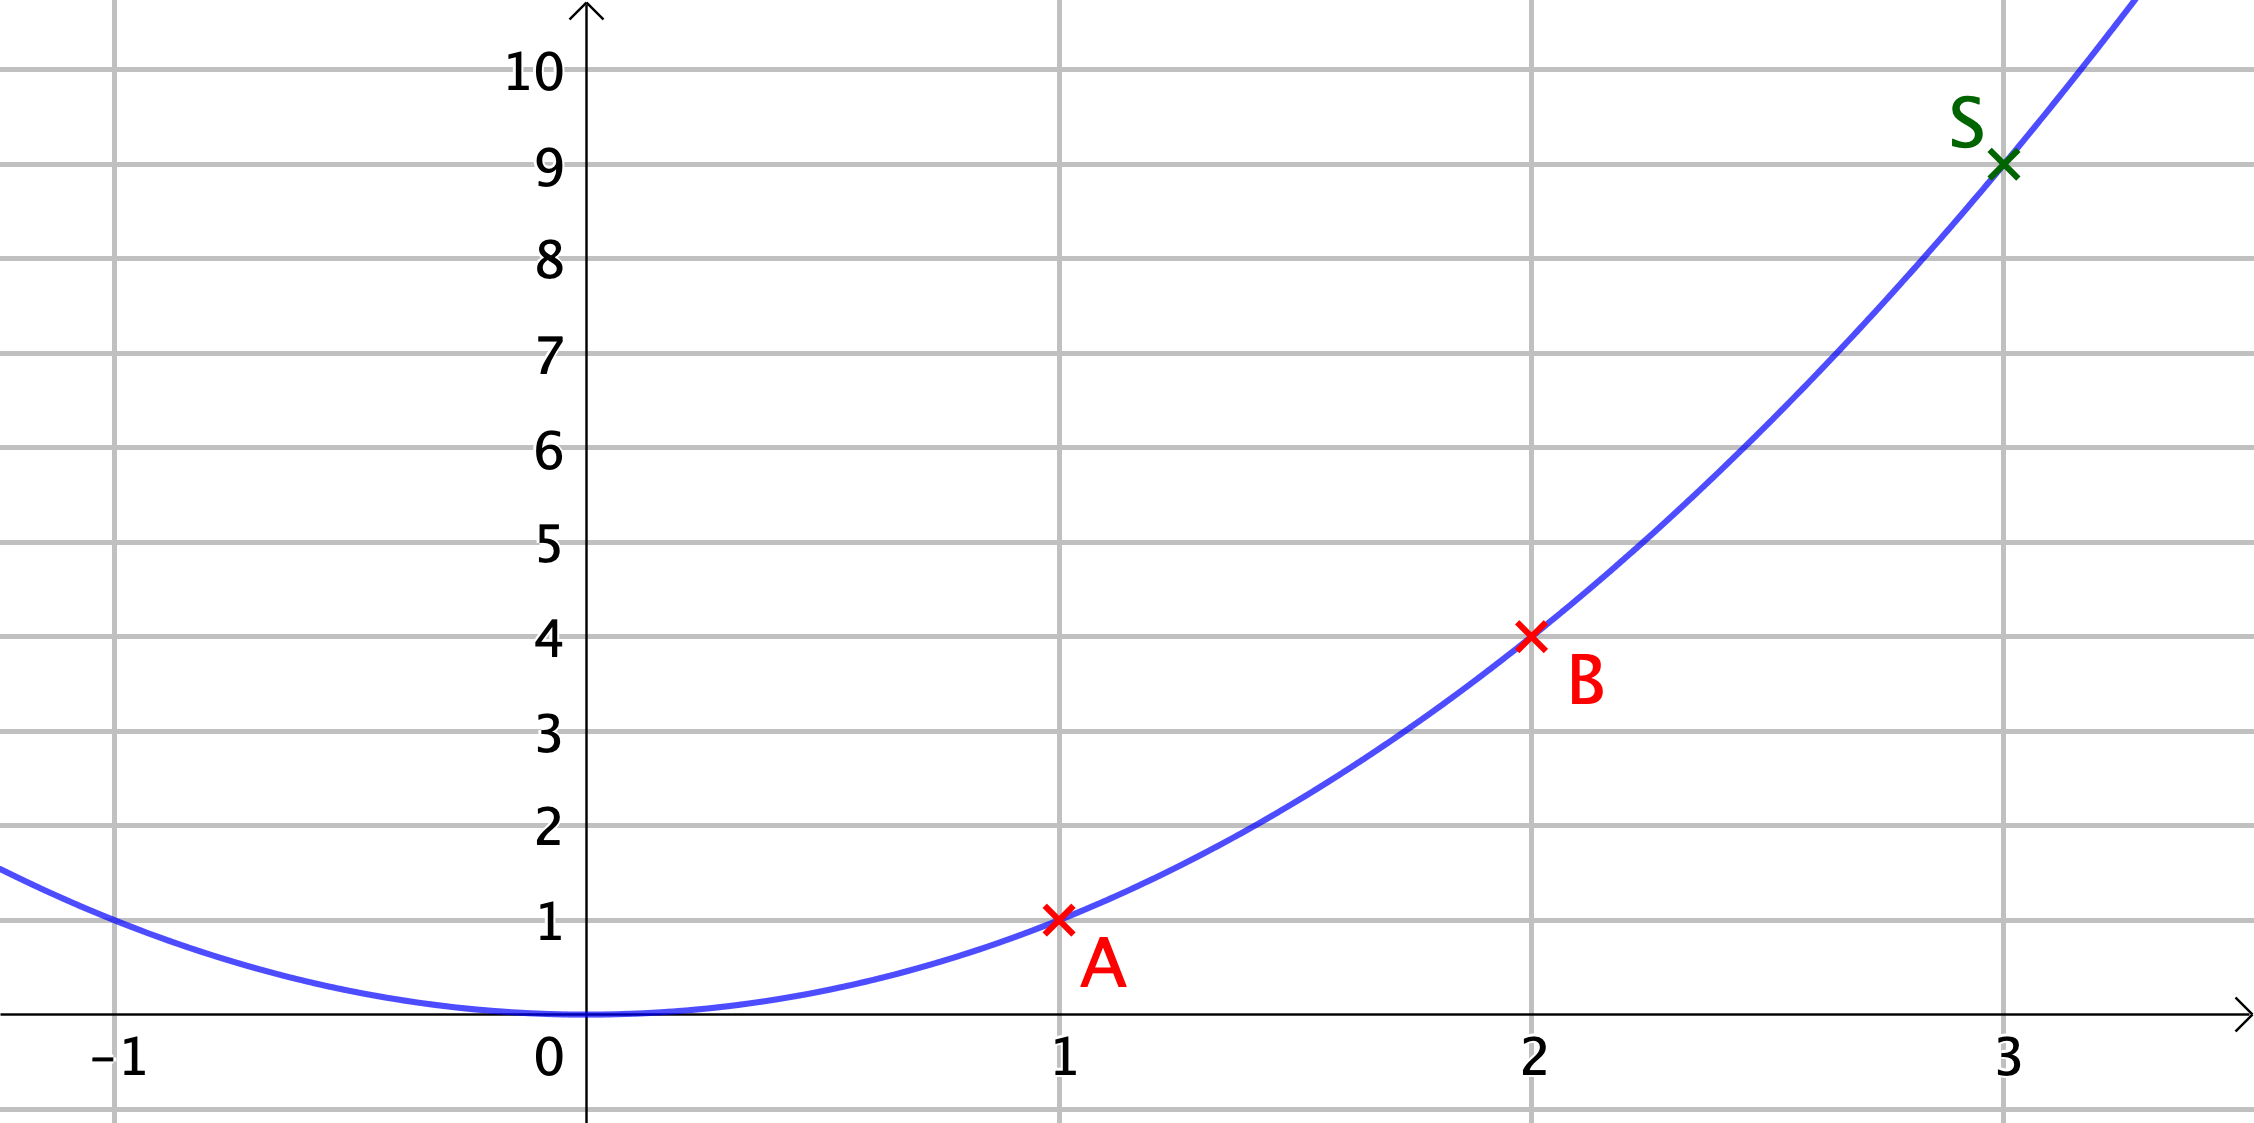
\includegraphics[scale = .8]{addition-on-parabolas/conjecture/a-and-b-positive.png}}
	
	\smallskip
	Cas où $a > 0$ et $b > 0$

	\columnbreak
	
	\fbox{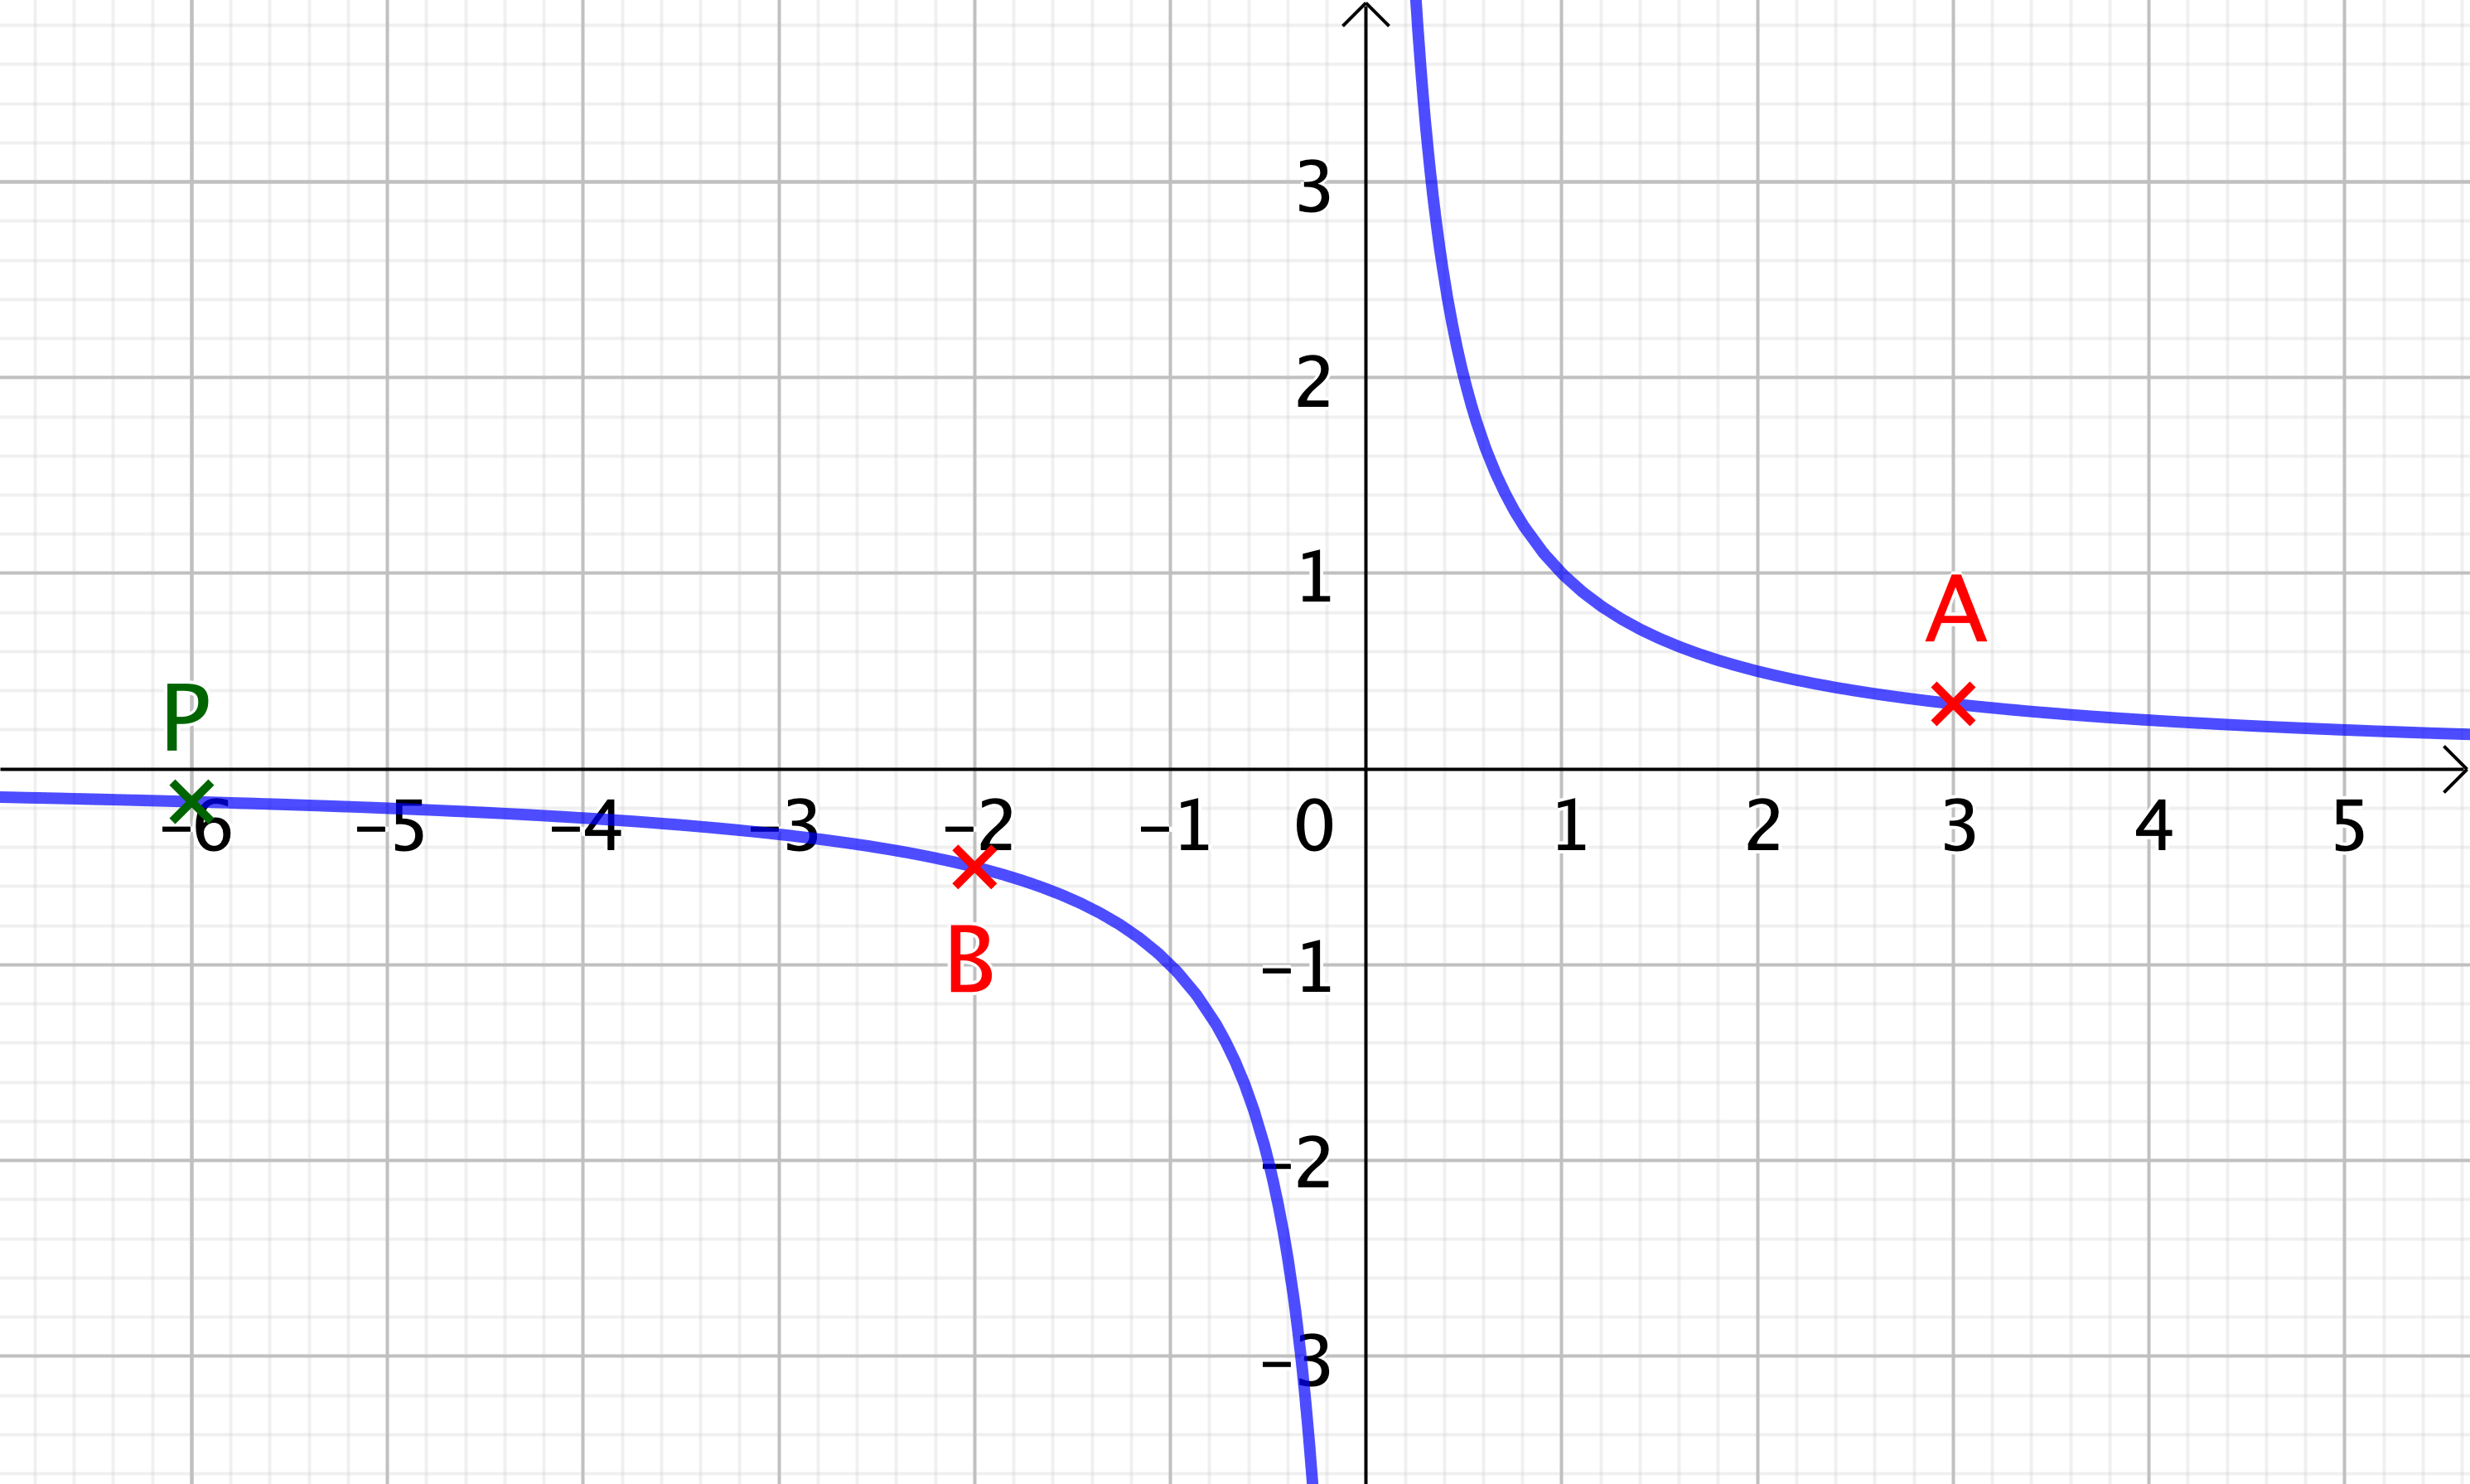
\includegraphics[scale = .8]{addition-on-parabolas/conjecture/a-and-b-diff-signs.png}}
	
	\smallskip
	Cas où $a < 0$ et $b > 0$
\end{multicols}
	
\begin{center}
	\footnotesize
	\itshape

	\fbox{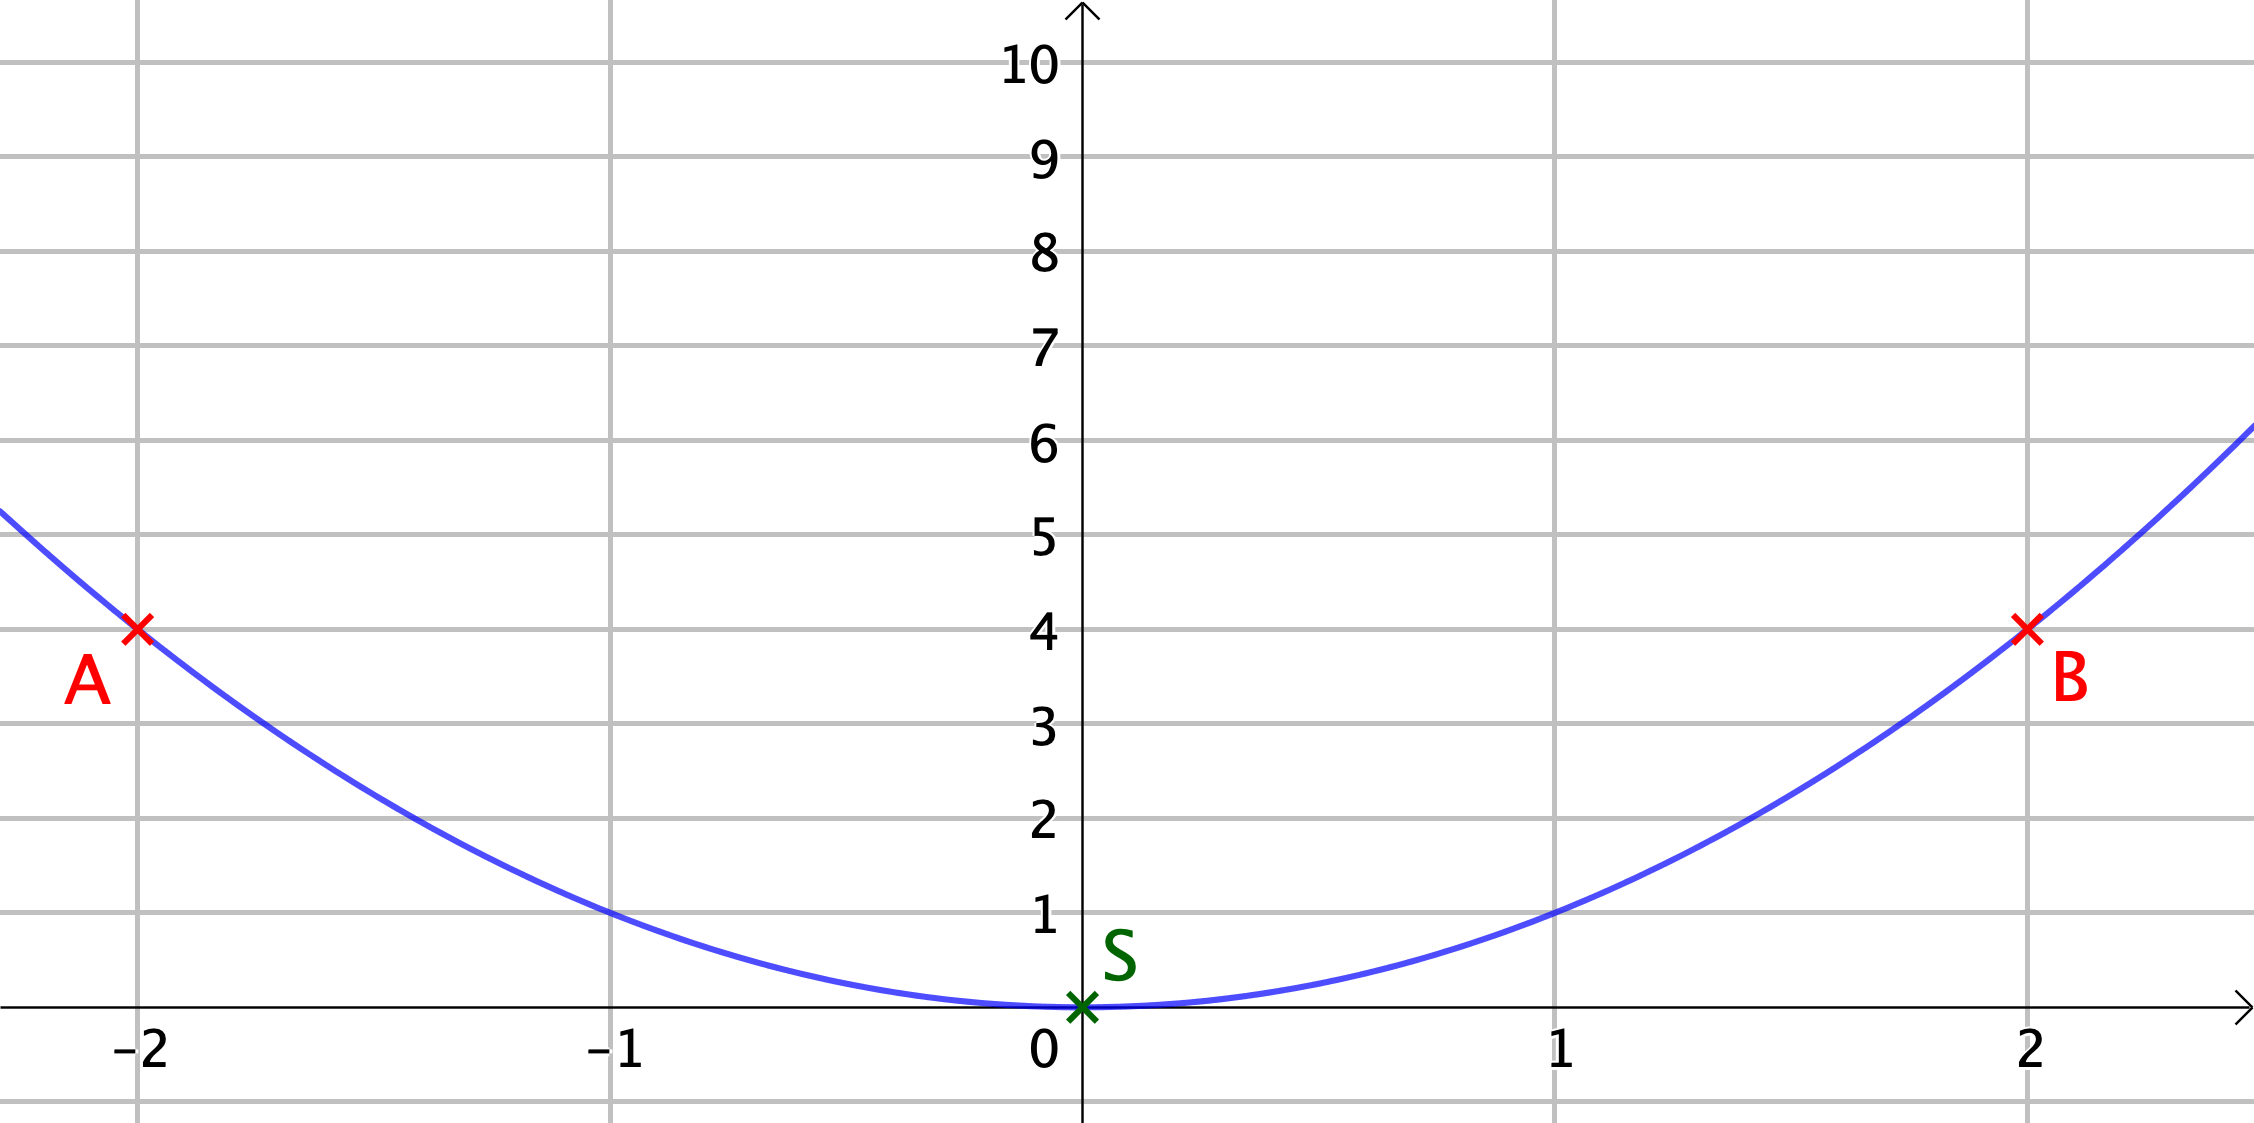
\includegraphics[scale = .8]{addition-on-parabolas/conjecture/a-and-b-opposite.png}}
	
	\smallskip
	Cas où $a = -b$
\end{center}


\newpage

Pour mieux voir ce qu'il se passe, traçons quelques droites. Voici ce que cela donne.

\begin{multicols}{2}
	\center
	\footnotesize
	\itshape

	\fbox{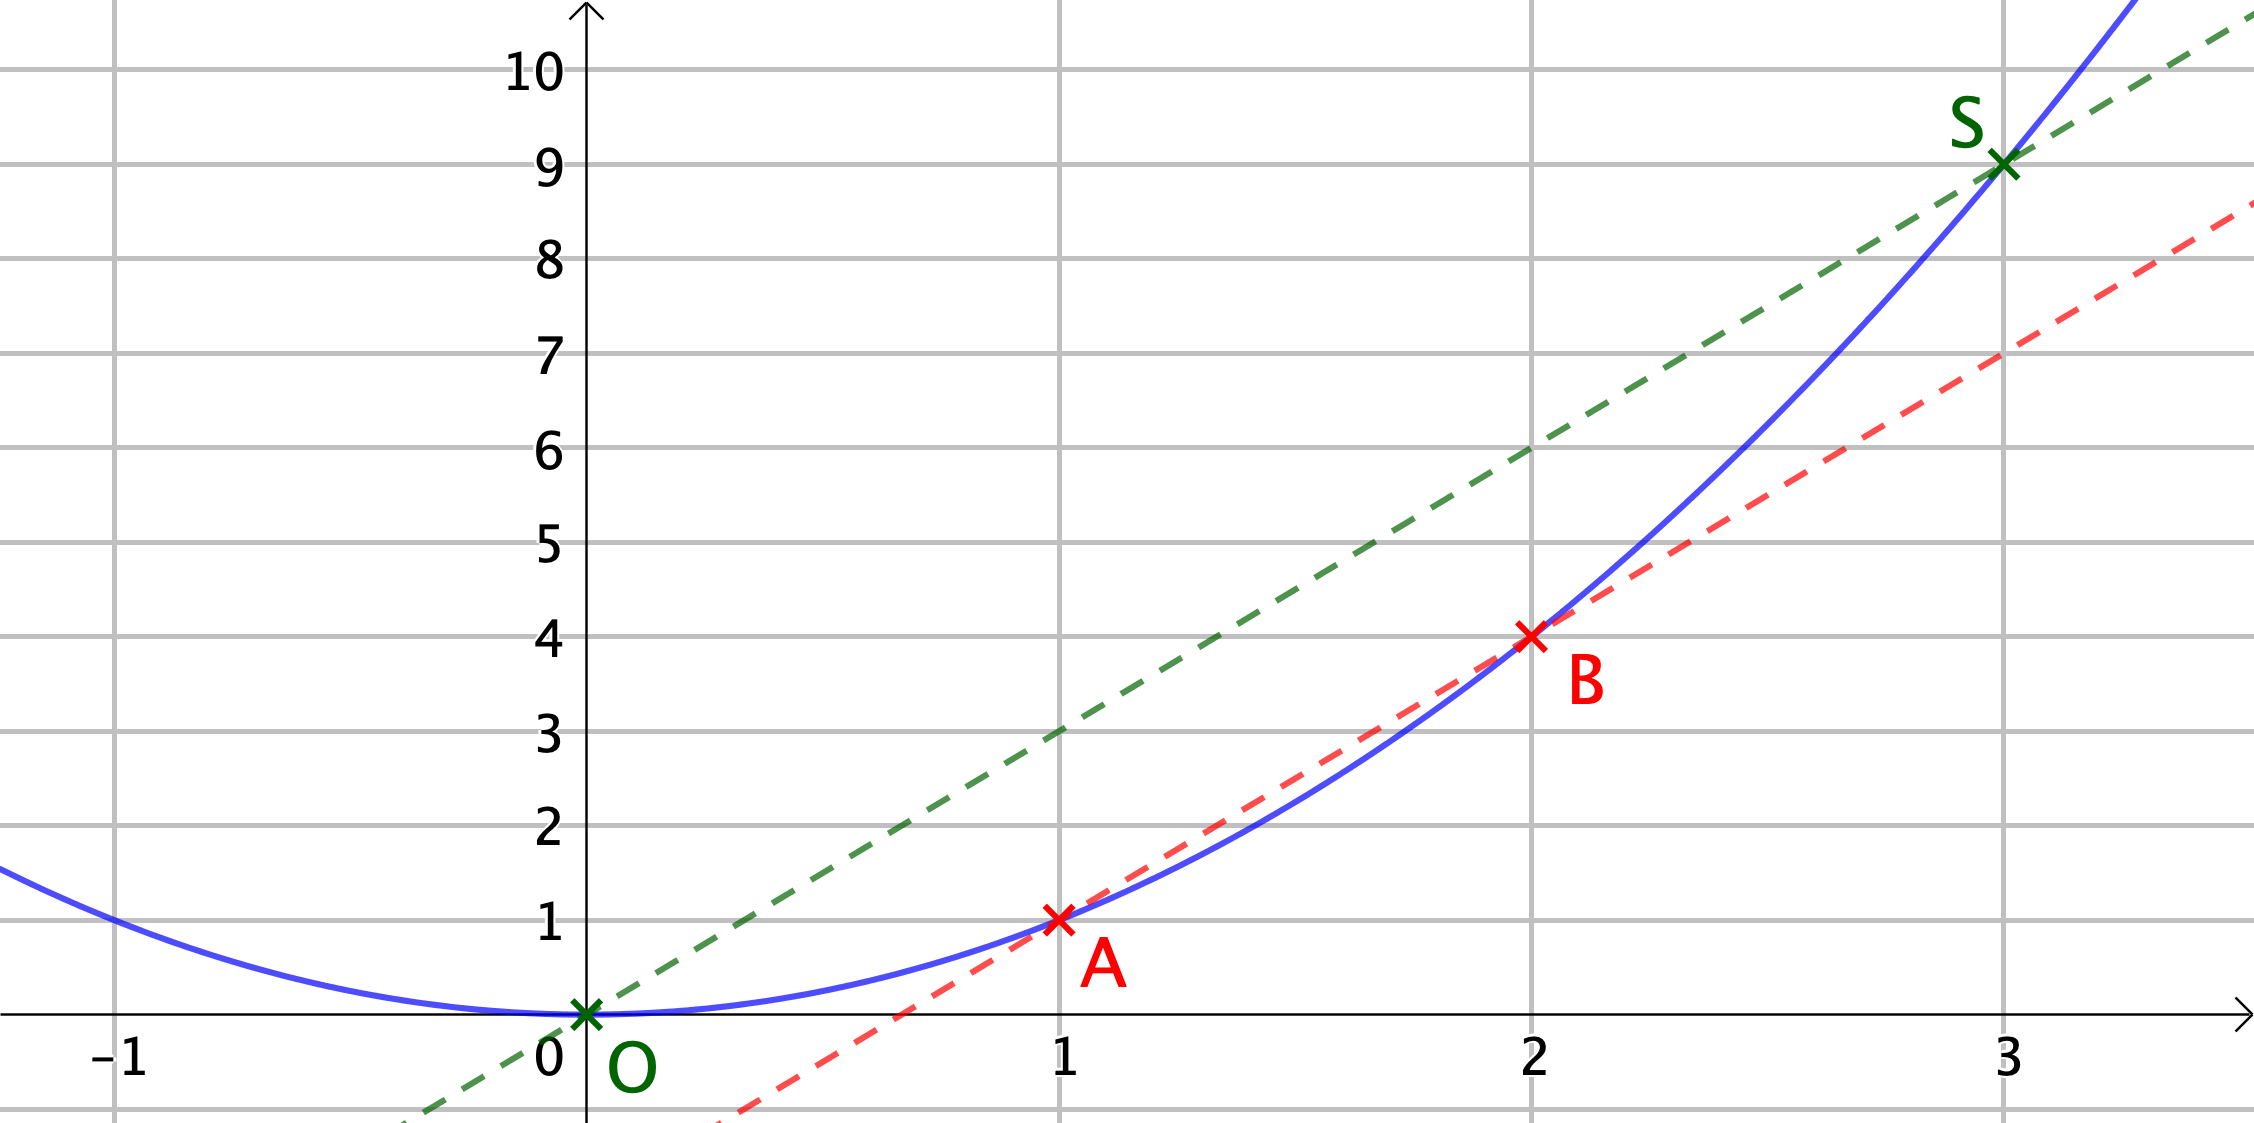
\includegraphics[scale = .8]{addition-on-parabolas/conjecture/a-and-b-positive-with-lines.png}}
	
	\smallskip
	Cas où $a > 0$ et $b > 0$

	\columnbreak
	
	\fbox{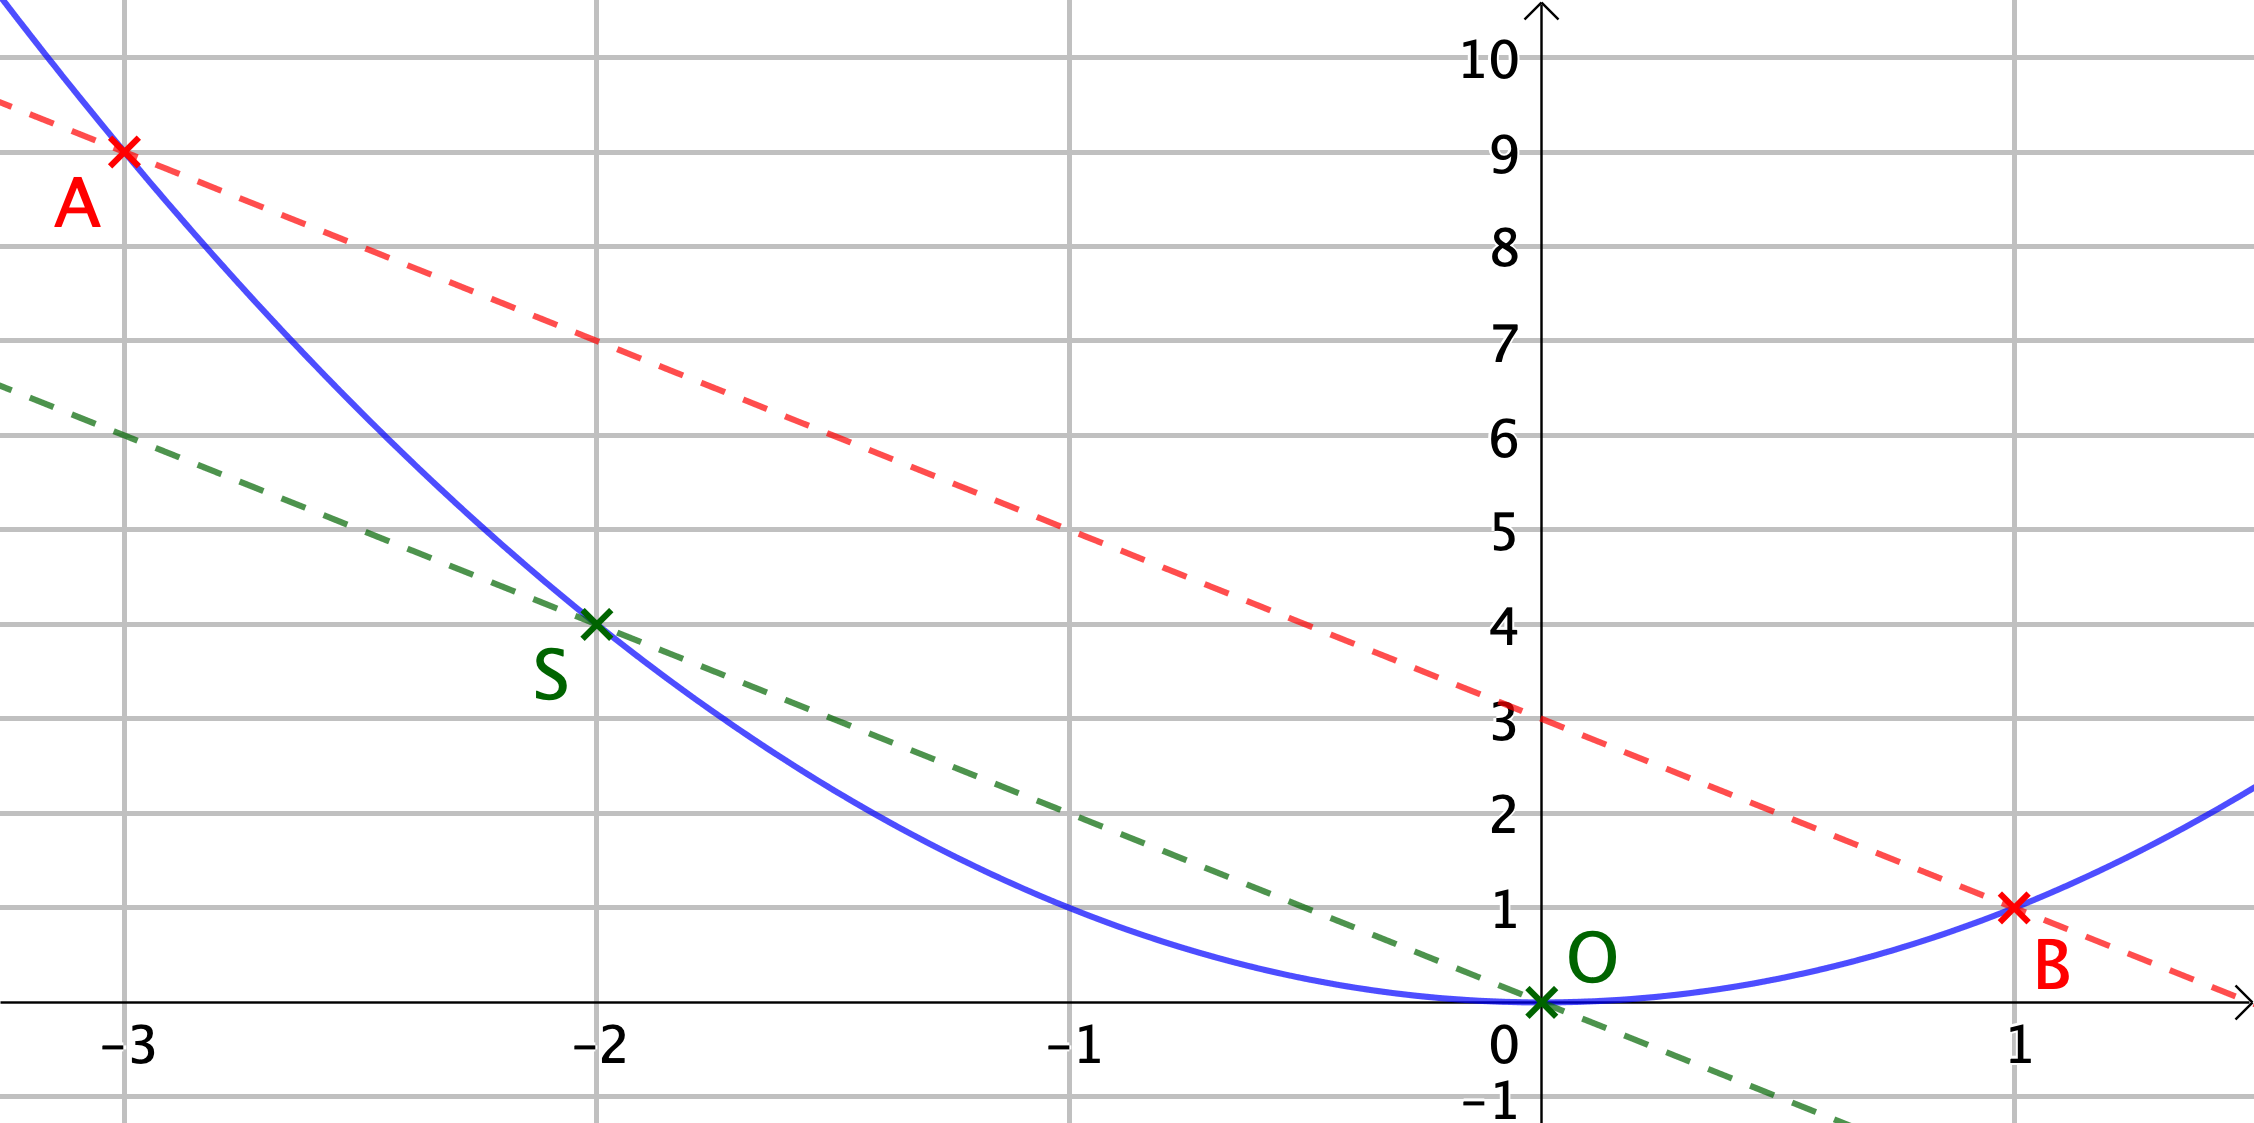
\includegraphics[scale = .8]{addition-on-parabolas/conjecture/a-and-b-diff-signs-with-lines.png}}
	
	\smallskip
	Cas où $a < 0$ et $b > 0$
\end{multicols}
	
\begin{center}
	\footnotesize
	\itshape

	\fbox{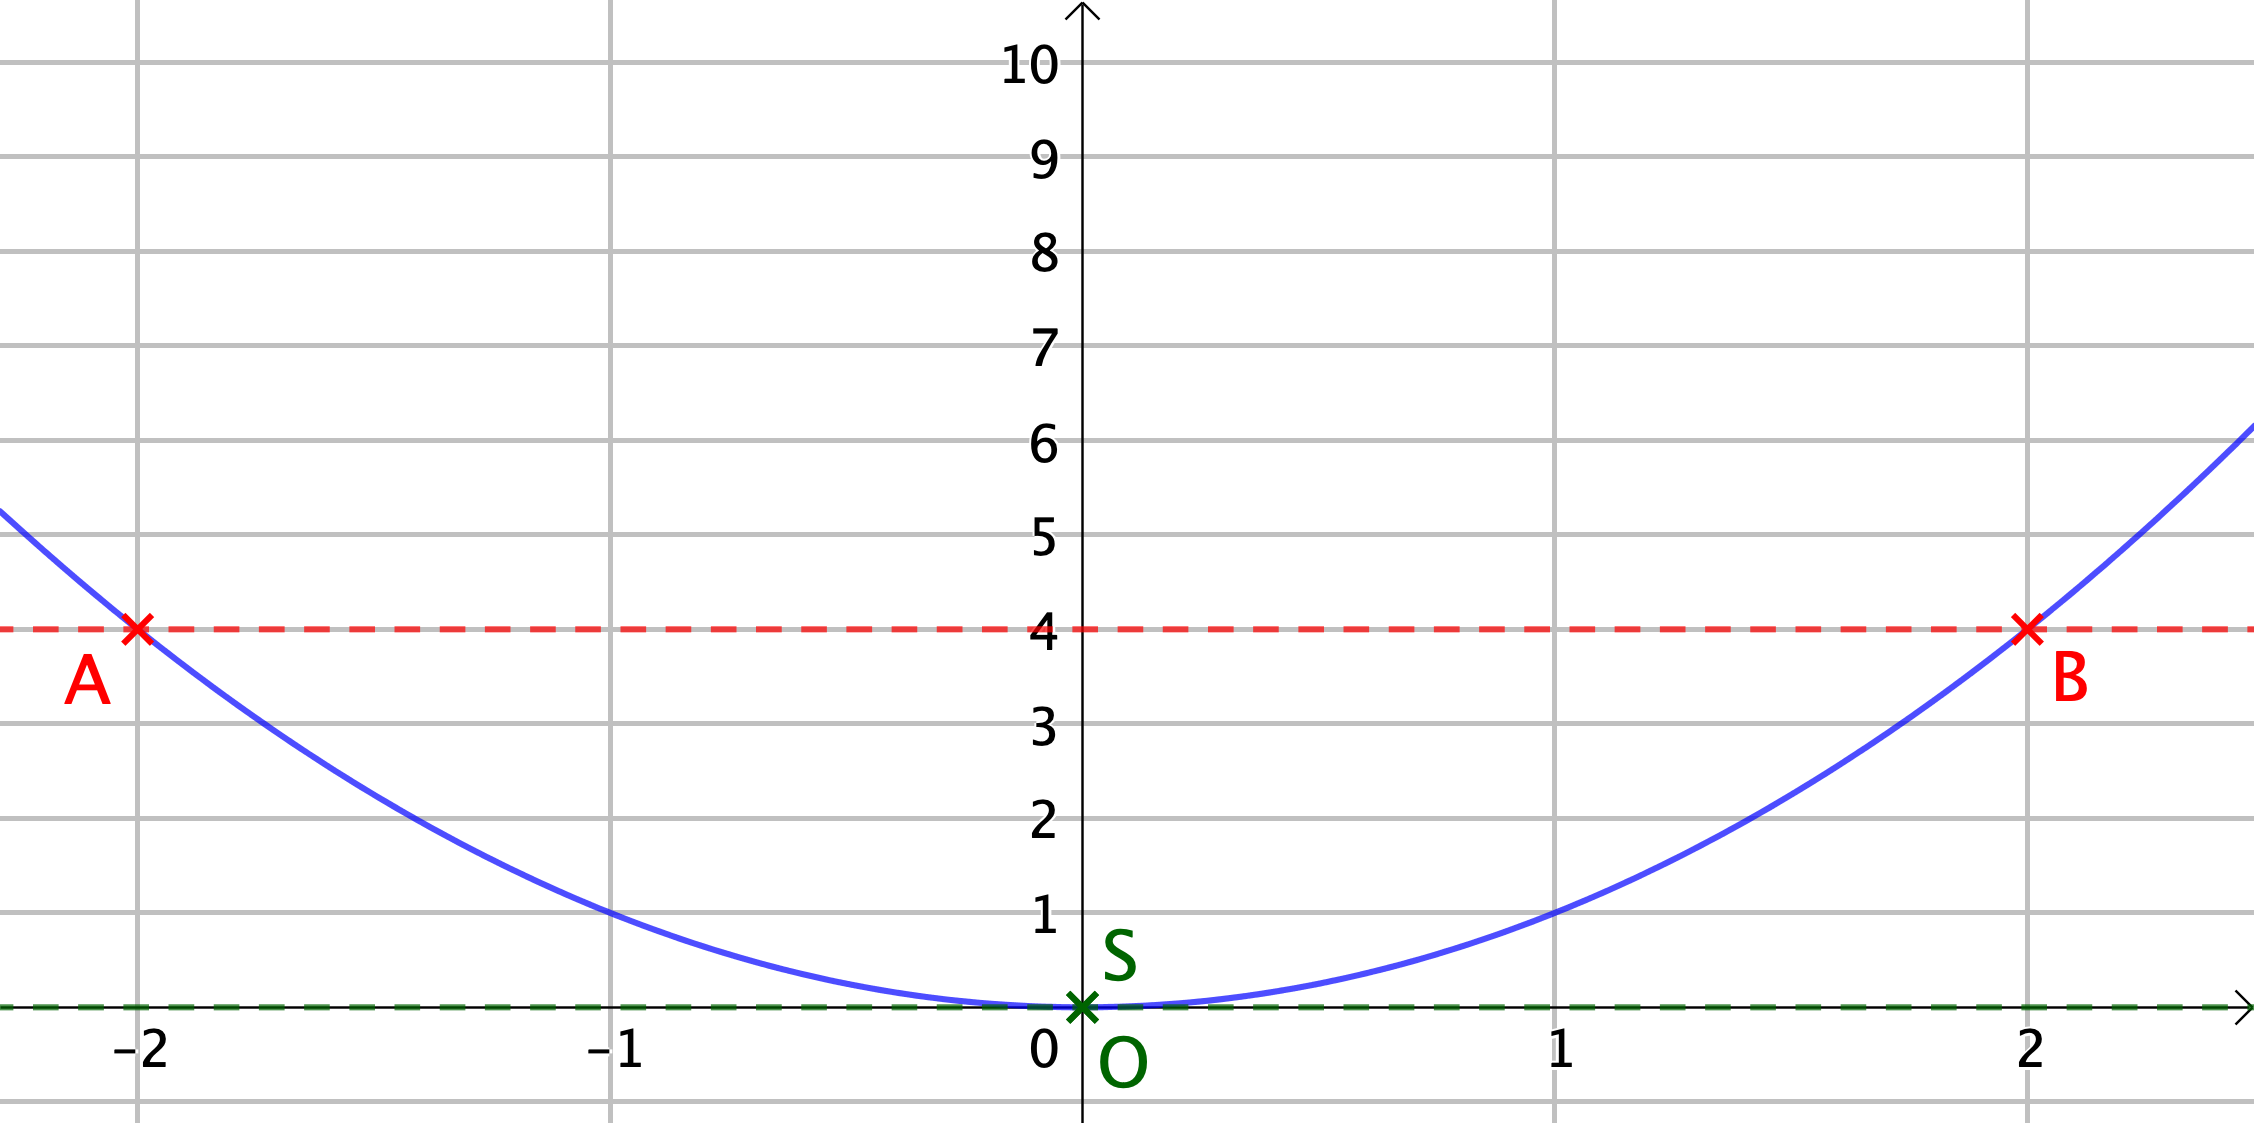
\includegraphics[scale = .8]{addition-on-parabolas/conjecture/a-and-b-opposite-with-lines.png}}
	
	\smallskip
	Cas où $a = -b$
\end{center}


\medskip

Il devient évident de conjecturer que le point $S$ se construit géométriquement comme suit.

\begin{enumerate}
	\item \label{point-1} Si $x_A \neq \pm \, x_B$ alors on construit la parallèle à $(AB)$ passant par $O$ l'origine du repère. Le point $S$ est le second point d'intersection de cette parallèle avec $\setgeo{P}$  \emph{(notons qu'une droite coupe $\setgeo{P}$ en au plus deux points)}.

	\item Si $x_A = - x_B$ alors $S = O$ . Notons au passage que l'on peut voir ceci comme un cas limite du précédent avec un point d'intersection \squote{double}.

	\item Si $x_A = x_B \neq 0$ , on procède comme au point (\ref{point-1}) mais avec la parallèle à la tangente en $A$ à la parabole $\setgeo{P}$ .
\end{enumerate}


La section qui suit va valider cette conjecture qui donne un moyen très capillotracté de calculer une somme de deux réels via la parabole $\setgeo{P}$ .
Plus sérieusement, la construction ci-dessus est une propriété géométrique très jolie de la parabole $\setgeo{P}$ .




\section{Preuve de la validité de la conjecture} \label{proof}

Revenons à nos entiers signés écrits sur $8$ bits en reprenant le calcul de $84 - 101 = -17$ tout en nous inspirant de ce qui a été vu dans la section précédente avec la base $10$.
Ici $256 = 2^8$ joue le même rôle que $1000 = 10^3$ avant. Nous avons ajouté des cases grises pour le bit du calcul intermédiaire, et nous avons indiqué les complémentations
\footnote{
	Nous utiliserons \emph{\og complémentation \fg} comme abréviation de \emph{\og complément à $2$ plus un \fg}. 
}
en mettant sur fond vert les bits les plus à gauche..

\medskip

\begin{center}
\begin{tabular}{ll}
	    & \!\!\binary{Za1010100}  	\\
	$-$ & \!\!\binary{Za1100101} 	\\[.8ex]
	\hline
	\hline 							\\[-2ex]
	    & \!\!\binary{Za1010100} 	\\
	$+$ & \!\!\binary{*a0011011} 	\\[.8ex]
	\hline \\[-2ex]
	$=$ & \!\!\binary{Uz1101111} 	\\[.8ex]
	\hline
	\hline 							\\[-2ex]
	$-$ & \!\!\binary{ca0010001} 	\\
\end{tabular}
\end{center}

\medskip

La dernière complémentation avec ajout d'un signe vient du $0$ sur fond gris et du fait qu'une seule complémentation préparatoire a été faite avant.
Tout s'éclaire !


\smallskip

Reprenons de même le cas de $84 - 61 = 23$ où l'on avait une retenue à ignorer. On fait comme précédemment.

\medskip

\begin{center}
\begin{tabular}{ll}
	    & \!\!\binary{Za1010100}  	\\
	$-$ & \!\!\binary{Za0111101} 	\\[.8ex]
	\hline
	\hline 							\\[-2ex]
	    & \!\!\binary{Za1010100} 	\\
	$+$ & \!\!\binary{*a1000011} 	\\[.8ex]
	\hline \\[-2ex]
	$=$ & \!\!\binary{Uu0010111} 	\\[.8ex]
	\hline
	\hline 							\\[-2ex]
	$+$ & \!\!\binary{Za0010111} 	\\
\end{tabular}
\end{center}

\medskip

Avec le nouvel éclairage, nous n'avons qu'à garder les bits sur fond blanc, le signe du résultat étant positif
\footnote{
	Il y a eu une seule complémentation préparatoire et le bit intermédiaire est $1$.
}.


\smallskip


Dans les deux cas précédents, au lieu de considérer un bit intermédiaire, il suffit d'effectuer directement le calcul de retenue sur le bit de gauche modulo $2$, ce calcul traduisant celui sur le nombre de complémentations préparatoires et du chiffre intermédiaire en gris dans nos deux exemples ci-dessus. On peut ainsi faire plus directement comme suit.
\begin{multicols}{2}
\begin{center}
\begin{tabular}{ll}
	    & \!\!\binary{Z1010100}  	\\
	$-$ & \!\!\binary{Z1100101} 	\\[.8ex]
	\hline
	\hline 							\\[-2ex]
	    & \!\!\binary{Z1010100} 	\\
	$+$ & \!\!\binary{*0011011} 	\\[.8ex]
	\hline \\[-2ex]
	$=$ & \!\!\binary{U1101111} 	\\[.8ex]
	\hline
	\hline 							\\[-2ex]
	$-$ & \!\!\binary{c0010001} 	\\
\end{tabular}
\end{center}

\null\vfill

\columnbreak

\begin{center}
\begin{tabular}{ll}
	    & \!\!\binary{Z1010100}  	\\
	$-$ & \!\!\binary{Z0111101} 	\\[.8ex]
	\hline
	\hline 							\\[-2ex]
	    & \!\!\binary{Z1010100} 	\\
	$+$ & \!\!\binary{*1000011} 	\\[.8ex]
	\hline \\[-2ex]
	$=$ & \!\!\binary{Z0010111} 	\\[.8ex]
	\hline
	\hline 							\\[-2ex]
	$+$ & \!\!\binary{Z0010111} 	\\
\end{tabular}
\end{center}
\end{multicols}






\smallskip

Plus généralement, avec la façon de stocker les entiers signés, nous avons alors les correspondances suivantes où les entiers additionnés $a$ et $b$ sont dans $\intervalC{-128}{127}$ et leur somme aussi, ce qui revient à ne considérer que les cas de non dépassement de capacité.
\begin{multicols}{4}
    \begin{center}
	\begin{tabular}{ll}
	    & \!\!\binary{Z-}  		\\
	$-$ & \!\!\binary{Z-} 		\\[.8ex]
	\hline
	\hline 						\\[-2ex]
	    & \!\!\binary{Z-} 		\\
	$+$ & \!\!\binary{*-} 		\\[.8ex]
	\hline \\[-2ex]
	$=$ & \!\!\binary{Z-} 	    \\
	\end{tabular}
	
	\medskip\itshape\footnotesize
	
	Soustraction 1
	
	de deux naturels
	\end{center}


	\null\vfill
	\columnbreak
	
	
	\begin{center}
	\begin{tabular}{ll}
	    & \!\!\binary{Z-}  		\\
	$-$ & \!\!\binary{Z-} 		\\[.8ex]
	\hline
	\hline 						\\[-2ex]
	    & \!\!\binary{Z-} 		\\
	$+$ & \!\!\binary{*-} 		\\[.8ex]
	\hline \\[-2ex]
	$=$ & \!\!\binary{U-} 	\\
	\end{tabular}
	
	\medskip\itshape\footnotesize
	
	Soustraction 2
	
	de deux naturels
	\end{center}


	\null\vfill
	\columnbreak
	
	
	\begin{center}
	\begin{tabular}{ll}
	$-$ & \!\!\binary{Z-}  		\\
	$-$ & \!\!\binary{Z-} 		\\[.8ex]
	\hline
	\hline 						\\[-2ex]
	    & \!\!\binary{*-} 		\\
	$+$ & \!\!\binary{*-} 		\\[.8ex]
	\hline \\[-2ex]
	$=$ & \!\!\binary{Z-} 	\\
	\end{tabular}
	
	\medskip\itshape\footnotesize
	
	Addition 1 de
	
	deux relatifs négatifs
	\end{center}


	\null\vfill
	\columnbreak
	
	
	\begin{center}
	\begin{tabular}{ll}
	$-$ & \!\!\binary{Z-}  		\\
	$-$ & \!\!\binary{Z-} 		\\[.8ex]
	\hline
	\hline 						\\[-2ex]
	    & \!\!\binary{*-} 		\\
	$+$ & \!\!\binary{*-} 		\\[.8ex]
	\hline \\[-2ex]
	$=$ & \!\!\binary{U-} 	\\
	\end{tabular}
	
	\medskip\itshape\footnotesize
	
	Addition 2 de
	
	deux relatifs négatifs
	\end{center}


	\null\vfill
\end{multicols}

\vspace{-1.5em}

Les soustractions et l'addition 2 ne posent aucun souci.
Par contre l'addition 1 est problématique avec son résultat positif. 
En fait cette addition contredit notre hypothèse de non dépassement de capacité. Nous allons voir pourquoi.

\medskip

Le cas de l'addition 1 correspond à $(a ; b) \in \intervalC{-128}{-1}^2$ tel que $(128 + a) + (128 + b) \in \intervalC{0}{127}$ soit $0 \leq 256 + a + b \leq 127$ \emph{i.e.} $-256 \leq a + b \leq -129$ ce qui correspond à un dépassement de capacité comme annoncé.
 
\medskip

Ceci achève de démontrer la validité des procédés d'addition et de soustraction d'entiers signés dans les cas de non dépassement de capacité.
Notez que le cas évident d'une addition de deux naturels a été omis, et aussi que $-a + b = b - a = b + (-a)$ et le fait qu'un changement de signe n'est autre qu'un complément à $1$ plus $1$ permettent de compléter les cas non indiqués ci-dessus.

\begin{exercise}
	Étudiez plus généralement le cas d'une base $b \in \NN_{\geq 3}$ quelconque.
\end{exercise}





\section{\texorpdfstring{Toute hyperbole d'équation $y = \frac{a x + b}{c x + d}$ a une structure de groupe}%
                        {Toute hyperbole d'équation y = (a x + b) / (c x + d) a une structure de groupe}}

Dans les preuves des sections précédentes, on constate que la construction géométrique se traduit par une identité basique qui est la clé de la périodicité de la suite de points $\left( A_i \right)$ . 
\begin{enumerate}
	\item Pour le cercle, c'était $\theta_i + \theta_{i+1} = \theta_{i+3} + \theta_{i+4}$ avec $\theta_i = \vangleorient{OI}{OA_i}$ . Nous nous intéressons ici juste à la 2\ieme preuve donnée dans la section \ref{circle-proof-2}. 

	\item Pour la parabole, c'était $x_i + x_{i+1} = x_{i+3} + x_{i+4}$ avec $x_k \in \RR$ des abscisses. 

	\item Pour l'hyperbole, c'était  $x_i x_{i+1} = x_{i+3} x_{i+4}$ avec $x_k \in \RRs$ des abscisses.
\end{enumerate}


\medskip


En fait, si $\Gamma$ désigne une ellipse, une parabole quelconque, ou une hyperbole quelconque, on peut démontrer l'existence d'un point $E \in \Gamma$ tel que la construction qui à $A \in \Gamma$ et $B \in \Gamma$ associe le point $S$ tel que $\setgeo*{C}{AB} \,/\!/\, \setgeo*{C}{ES}$ définisse une loi de groupe $\star$ sur $\Gamma$ avec $E$ pour élément neutre. 
Les cas étudiés dans ce document n'en sont que des cas particuliers. 
Le lecteur intéressé peut se reporter à  
\emph{\og Faire des additions modulaires sur une ellipse \fg} ,
\emph{\og Faire des additions sur une parabole \fg} 
et
\emph{\og Faire des produits sur une hyperbole \fg}
qui ont été rédigés par l'auteur de ce document
\footnote{
	Voir \texttt{addition-on-ellipsis.pdf} , \texttt{addition-on-parabolas.pdf}  et \texttt{product-on-hyperbolas.pdf}  à l'adresse \url{https://github.com/bc-writing/drafts} .
}.


\medskip


Tout comme dans la preuve dans la section \ref{circle-proof-2} , on constate alors que la construction \emph{\og magique \fg} est telle que $\forall n \in \NN_{\geq 5}$ , $A_{n}$ est l'unique point de $\Gamma$ tel que $\setgeo*{C}{A_{n} A_{n-1}} \,/\!/\, \setgeo*{C}{A_{n-3} A_{n-4}}$ . On en déduit alors que $A_{n} \star A_{n-1} = A_{n-3} \star A_{n-4}$ . On retombe alors sur une identité similaire à celles redonnées ci-dessus mais avec la loi $\star$ au lieu des lois $+$ avec des angles orientés, $+$ avec des réels et $\times$ avec des réels non nuls. On conclut alors de la même façon. Que les mathématiques sont belles quand on prend le temps de les écouter !




% Voir si caractéristique : il transof complexe de 1/x vers x^2 uis on utiliserait cas complexe pour revenir à l'hyperbole . FAISABLE ???????
\end{document}
